\documentclass{beamer}
\graphicspath{ {img/} }

%Information to be included in the title page:
\title{MAPF project}
\author{Andrés Córdova and Aleksandra Khatova}
\institute{Unversity of Potsdam}
\date{2022}

\AtBeginSection[]
{
  \begin{frame}
    \frametitle{Table of Contents}
    \tableofcontents[currentsection]
  \end{frame}
}

\begin{document}
\frame{\titlepage}

\begin{frame}
\begin{itemize}
    \item Non-anonymous
    \item There is a path from each startig position to every shelf that do not pass through other shelves
    \item Rectangular grid
    \item One robot per shelf
    \item Density more than 5\% less than 50\%
\end{itemize}
\end{frame}

\begin{frame}
\frametitle{Warehouse-like instances}
\centering
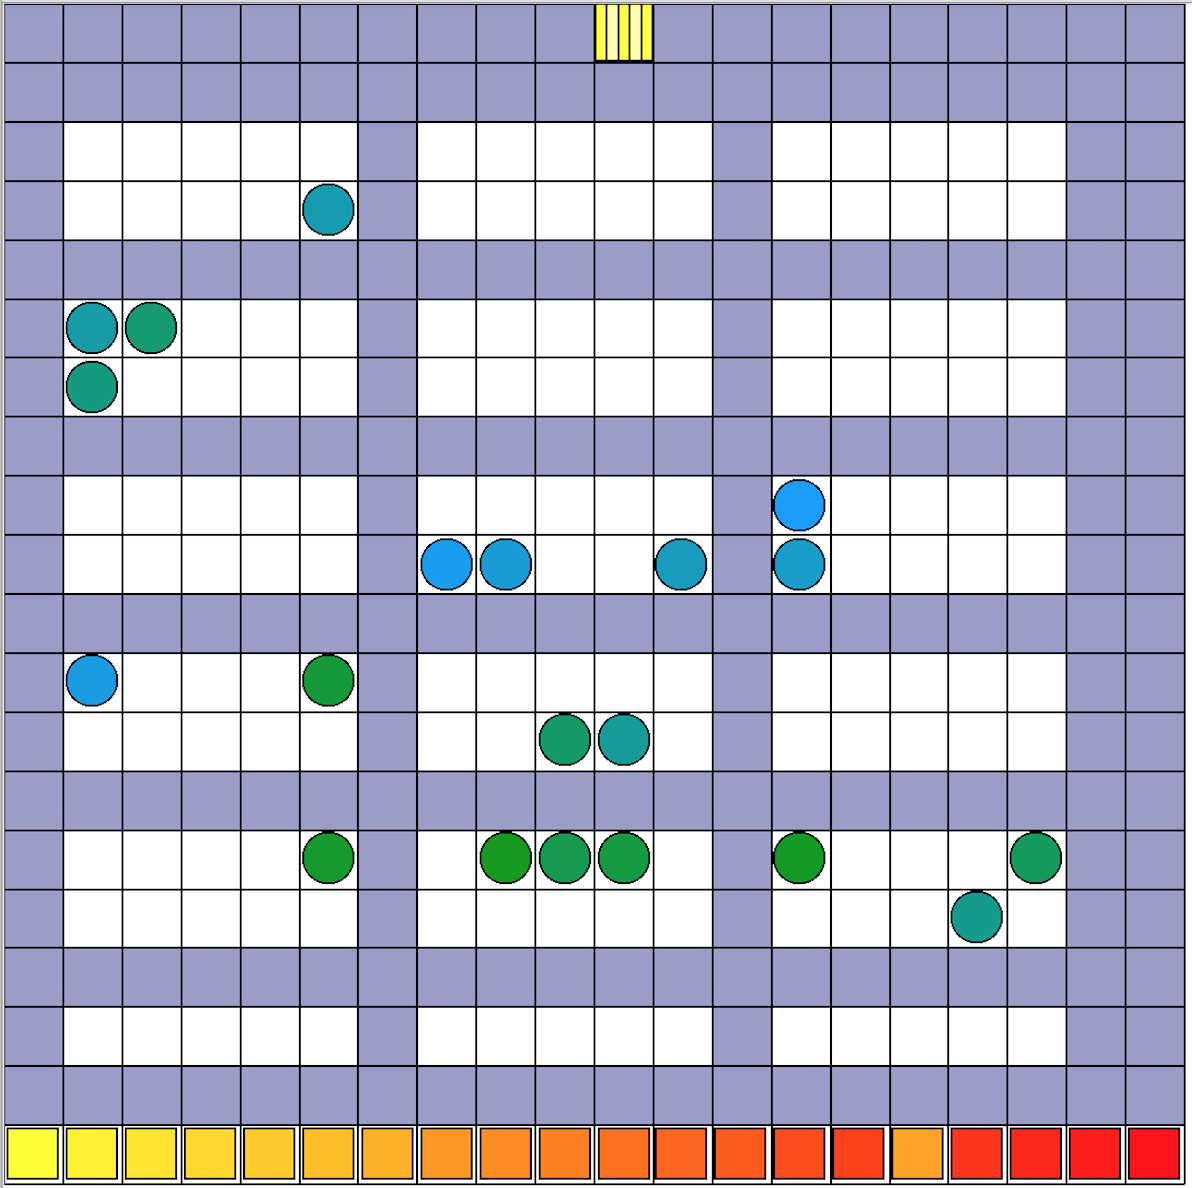
\includegraphics[scale=0.3]{med_dense.png}
\end{frame}

\begin{frame}
\frametitle{Types of solution}
\begin{itemize}
    \item Reduction-based solvers
    \item MAPF-specific sub-optimal solvers
    \item Search-based suboptimal solvers
    \item Rule-based suboptimal solvers
    \item Hybrid solvers
\end{itemize}
\end{frame}

\begin{frame}
\centering
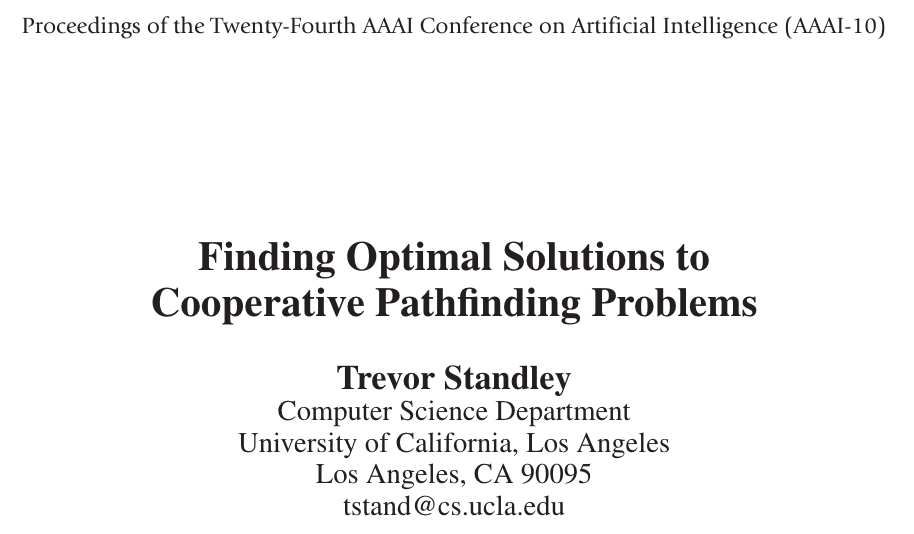
\includegraphics[scale=0.3]{OD+ID.png}
\end{frame}

\begin{frame}
\frametitle{OD+ID}
\begin{itemize} 
\item Independence detection
\item Operator decomposition
\end{itemize} 
\end{frame}

\begin{frame}
\frametitle{OD+ID}
\begin{itemize} 
\item Independence detection
\begin{enumerate}
\item $n$ agents $\implies$ $n$ paths $\implies$ $n$ groups (groups contains paths)
\item $\forall (i,j), i \neq j$ if $path_i$ conflicts $path_j$ then $group_{ij} = \{path_i, path_j\}$, delete $group_i$, delete $group_j$
\item  if $group_i$ is unitary group then $path_i$ stays fixed in the final solution
\item Create illegal moves table: illegal((X,Y), T)
\item if $group$ has more than one element resolve conflicts of that group
\end{enumerate}
\item Operator decomposition
\end{itemize}
\end{frame}

\begin{frame}
\frametitle{OD+ID}
\begin{itemize} 
\item Independence detection
\item Operator decomposition
\begin{enumerate}
    \item cost(position(R),goal(R),T)
    \item state(position(R1,(X,Y),T), ...,position(RN,(X',Y'),T), move(R1,(DX,DY),T+1), move(RN,(DX',DY'),T+1))
    \item conflict avoidance table: avoidance((X,Y),T)
    \item move(R,(DX,DY),T+1) so cost(T+1) < cost(T) considering avoidance and illegal tables
\end{enumerate}
\end{itemize}
\end{frame}

\begin{frame}
\frametitle{OD+ID}
\begin{itemize} 
\item Advantages: Completeness, low computational cost
\item Disadvantages: Suboptimal, do not solve everything
\end{itemize} 
\end{frame}

\begin{frame}
\centering
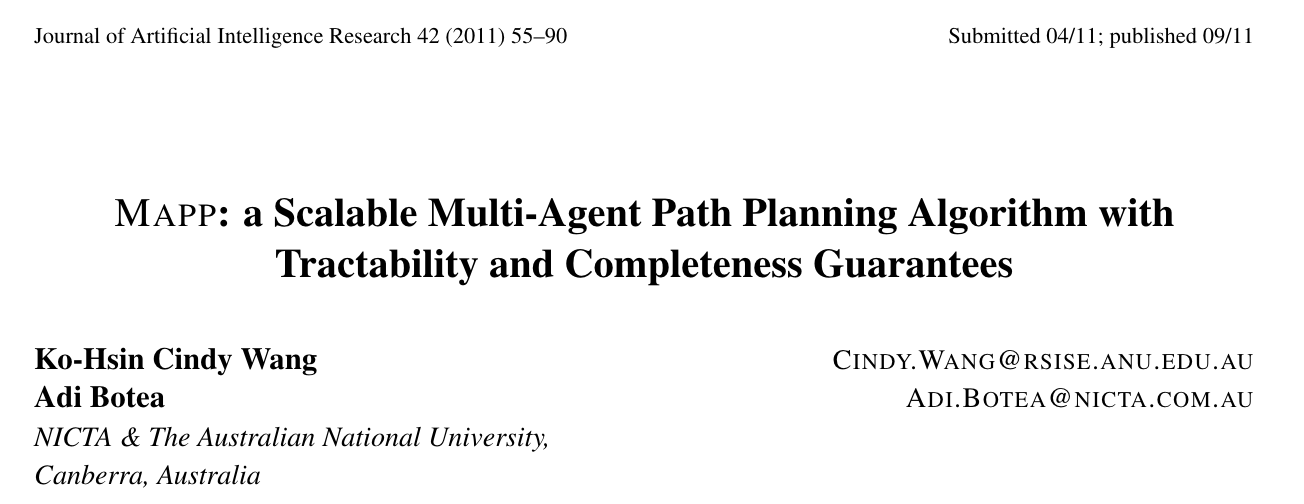
\includegraphics[scale=0.3]{MAPP.png}
\end{frame}

\begin{frame}
\frametitle{MAPP}
\centering
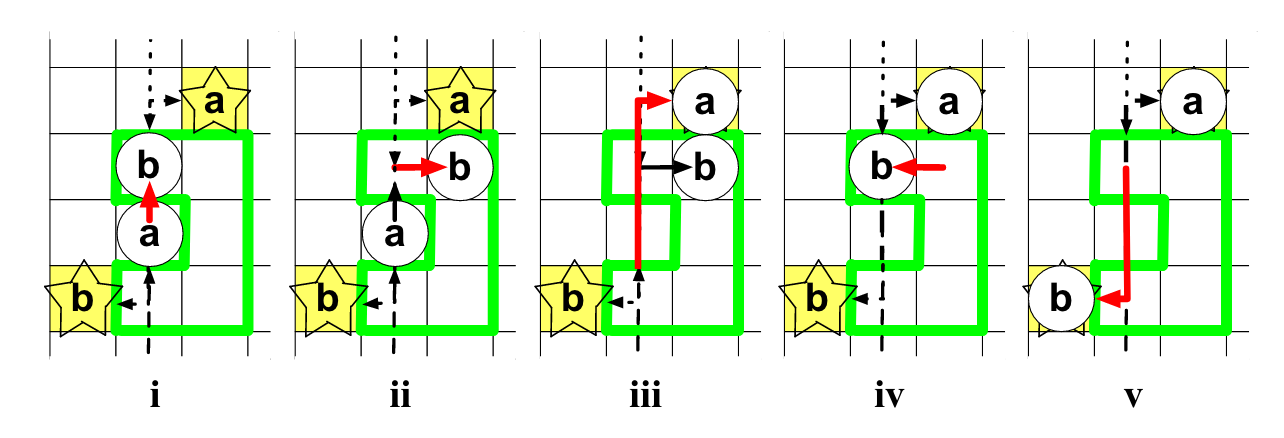
\includegraphics[scale=0.47]{MAPP_example.png}
\begin{itemize} 
\item Blank travel 
\item Alternative paths
\item Private zones
\end{itemize} 
\end{frame}

\begin{frame}
\frametitle{MAPP: alternative paths}
Alternative paths characterize a map, not a particular solution
\centering
$$\downarrow $$
They have to be calculated only once for each map
\centering
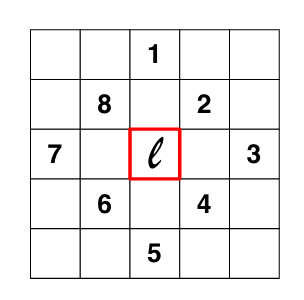
\includegraphics[scale=1.0]{MAPP_alt_paths.png}
\end{frame}

\begin{frame}
\frametitle{MAPP: blank travel}
If you always can do blank travel, then you can obtain a complete solution
$$\downarrow$$
Define a class of ``slidable'' instances where blank travel is always possible \\
\centering
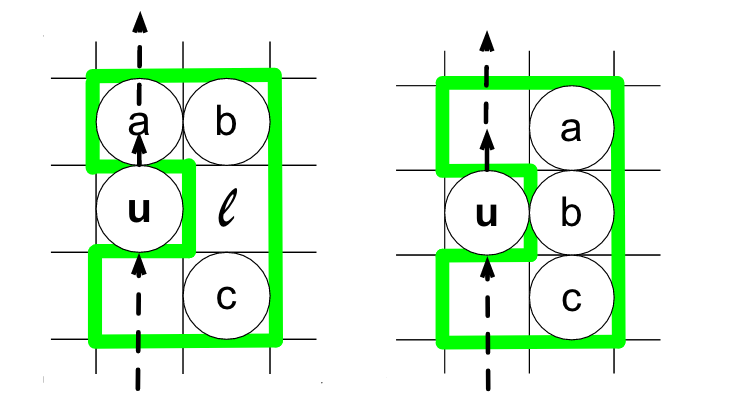
\includegraphics[scale=0.5]{MAPP_blank.png}
\end{frame}

\begin{frame}
\frametitle{MAPP}
\begin{itemize} 
\item Complete only for ``slidable'' instances 
\item Suboptimal
\item Can completely solve huge dense warehouse-like instances
\end{itemize} 
\end{frame}

\end{document}